\documentclass[border=10pt]{standalone}
\usepackage{tikz}\usepackage{amsmath}\usetikzlibrary{calc,arrows.meta,decorations.markings}
\begin{document}
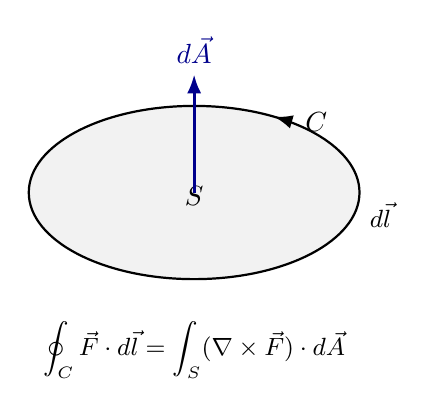
\begin{tikzpicture}[line width=0.9pt,>={Latex[length=2.4mm]}]
  % superficie (casquete) con borde C
  \draw[thick,fill=black!5,decoration={markings,mark=at position 0.15 with {\arrow{Latex}}},postaction={decorate}] (0,0) ellipse (2.1 and 1.1);
  \node at (0,-0.05){$S$};
  \node at (1.55,0.9){$C$};
  \node[below right] at (2.1,0){\small $d\vec l$};
  % normal dA (regla de la mano derecha)
  \draw[->,blue!55!black,line width=1.1pt] (0,0)--(0,1.5) node[above]{$d\vec A$};
  \node at (0,-2.0){\small $\displaystyle\oint_C \vec F\cdot d\vec l=\int_S (\nabla\times\vec F)\cdot d\vec A$};
\end{tikzpicture}
\end{document}
